\subsection{Glyph: \glyph{Biological activity}}
\label{af:sec:biologicalActivity}


\begin{glyphDescription}

\glyphSboTerm SBO:

\glyphContainer An \glyph{unspecified activity} is represented by an elliptic container, as shown in \fig{af:unspecified}.

\glyphLabel An \glyph{unspecified actifity} is identified by a label placed in an unbordered box containing a string of characters.  The characters can be distributed on several lines to improve readability, although this is not mandatory.  The label box must be attached to the center of the container.  The label may spill outside of the container.

\end{glyphDescription}

\begin{figure}[H]
  \centering
  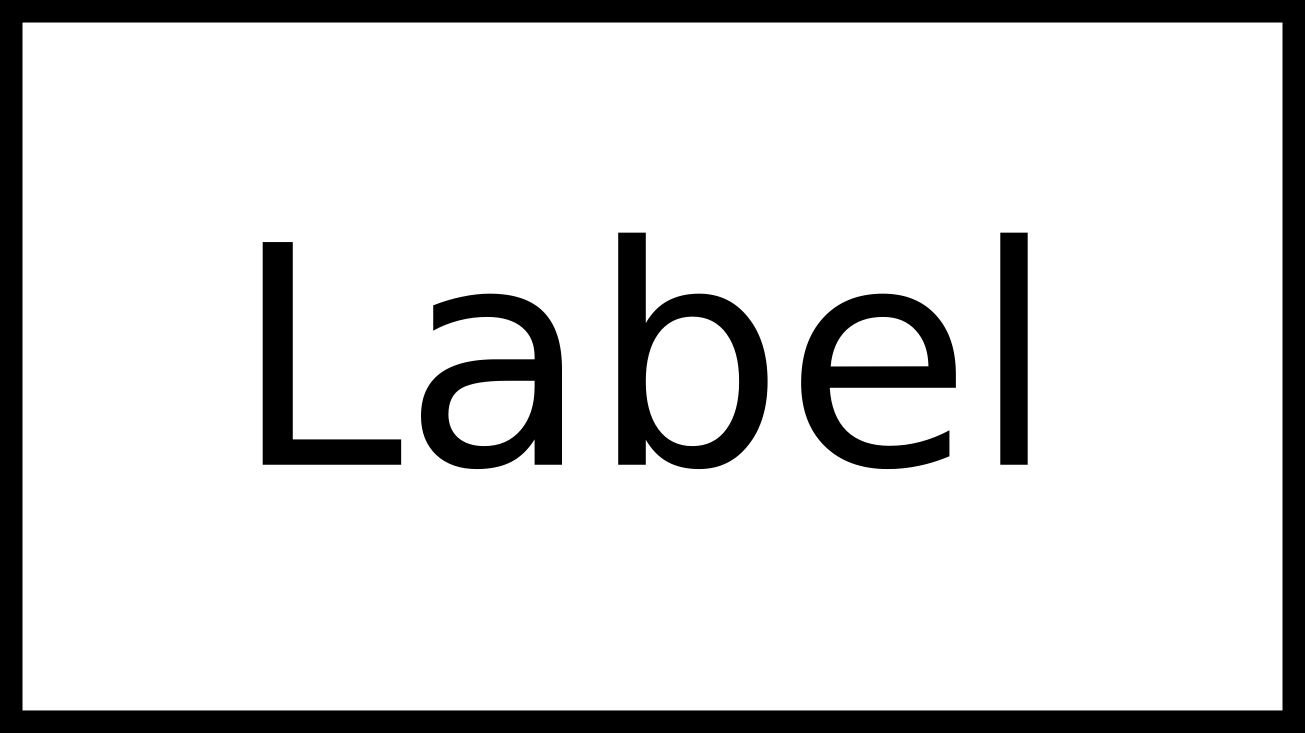
\includegraphics[scale = 0.3]{images/biologicalActivity}
  \caption{The \AF glyph for \glyph{biological activity}.}
  \label{fig:af:biologicalActivity}
\end{figure}
